% Options for packages loaded elsewhere
\PassOptionsToPackage{unicode}{hyperref}
\PassOptionsToPackage{hyphens}{url}
\PassOptionsToPackage{dvipsnames,svgnames,x11names}{xcolor}
%
\documentclass[
  dissertation]{bsu-cs}

\usepackage{amsmath,amssymb}
\usepackage{iftex}
\ifPDFTeX
  \usepackage[T1]{fontenc}
  \usepackage[utf8]{inputenc}
  \usepackage{textcomp} % provide euro and other symbols
\else % if luatex or xetex
  \usepackage{unicode-math}
  \defaultfontfeatures{Scale=MatchLowercase}
  \defaultfontfeatures[\rmfamily]{Ligatures=TeX,Scale=1}
\fi
\usepackage{lmodern}
\ifPDFTeX\else  
    % xetex/luatex font selection
\fi
% Use upquote if available, for straight quotes in verbatim environments
\IfFileExists{upquote.sty}{\usepackage{upquote}}{}
\IfFileExists{microtype.sty}{% use microtype if available
  \usepackage[]{microtype}
  \UseMicrotypeSet[protrusion]{basicmath} % disable protrusion for tt fonts
}{}
\usepackage{xcolor}
\setlength{\emergencystretch}{3em} % prevent overfull lines
\setcounter{secnumdepth}{-\maxdimen} % remove section numbering
% Make \paragraph and \subparagraph free-standing
\makeatletter
\ifx\paragraph\undefined\else
  \let\oldparagraph\paragraph
  \renewcommand{\paragraph}{
    \@ifstar
      \xxxParagraphStar
      \xxxParagraphNoStar
  }
  \newcommand{\xxxParagraphStar}[1]{\oldparagraph*{#1}\mbox{}}
  \newcommand{\xxxParagraphNoStar}[1]{\oldparagraph{#1}\mbox{}}
\fi
\ifx\subparagraph\undefined\else
  \let\oldsubparagraph\subparagraph
  \renewcommand{\subparagraph}{
    \@ifstar
      \xxxSubParagraphStar
      \xxxSubParagraphNoStar
  }
  \newcommand{\xxxSubParagraphStar}[1]{\oldsubparagraph*{#1}\mbox{}}
  \newcommand{\xxxSubParagraphNoStar}[1]{\oldsubparagraph{#1}\mbox{}}
\fi
\makeatother

\usepackage{color}
\usepackage{fancyvrb}
\newcommand{\VerbBar}{|}
\newcommand{\VERB}{\Verb[commandchars=\\\{\}]}
\DefineVerbatimEnvironment{Highlighting}{Verbatim}{commandchars=\\\{\}}
% Add ',fontsize=\small' for more characters per line
\usepackage{framed}
\definecolor{shadecolor}{RGB}{241,243,245}
\newenvironment{Shaded}{\begin{snugshade}}{\end{snugshade}}
\newcommand{\AlertTok}[1]{\textcolor[rgb]{0.68,0.00,0.00}{#1}}
\newcommand{\AnnotationTok}[1]{\textcolor[rgb]{0.37,0.37,0.37}{#1}}
\newcommand{\AttributeTok}[1]{\textcolor[rgb]{0.40,0.45,0.13}{#1}}
\newcommand{\BaseNTok}[1]{\textcolor[rgb]{0.68,0.00,0.00}{#1}}
\newcommand{\BuiltInTok}[1]{\textcolor[rgb]{0.00,0.23,0.31}{#1}}
\newcommand{\CharTok}[1]{\textcolor[rgb]{0.13,0.47,0.30}{#1}}
\newcommand{\CommentTok}[1]{\textcolor[rgb]{0.37,0.37,0.37}{#1}}
\newcommand{\CommentVarTok}[1]{\textcolor[rgb]{0.37,0.37,0.37}{\textit{#1}}}
\newcommand{\ConstantTok}[1]{\textcolor[rgb]{0.56,0.35,0.01}{#1}}
\newcommand{\ControlFlowTok}[1]{\textcolor[rgb]{0.00,0.23,0.31}{\textbf{#1}}}
\newcommand{\DataTypeTok}[1]{\textcolor[rgb]{0.68,0.00,0.00}{#1}}
\newcommand{\DecValTok}[1]{\textcolor[rgb]{0.68,0.00,0.00}{#1}}
\newcommand{\DocumentationTok}[1]{\textcolor[rgb]{0.37,0.37,0.37}{\textit{#1}}}
\newcommand{\ErrorTok}[1]{\textcolor[rgb]{0.68,0.00,0.00}{#1}}
\newcommand{\ExtensionTok}[1]{\textcolor[rgb]{0.00,0.23,0.31}{#1}}
\newcommand{\FloatTok}[1]{\textcolor[rgb]{0.68,0.00,0.00}{#1}}
\newcommand{\FunctionTok}[1]{\textcolor[rgb]{0.28,0.35,0.67}{#1}}
\newcommand{\ImportTok}[1]{\textcolor[rgb]{0.00,0.46,0.62}{#1}}
\newcommand{\InformationTok}[1]{\textcolor[rgb]{0.37,0.37,0.37}{#1}}
\newcommand{\KeywordTok}[1]{\textcolor[rgb]{0.00,0.23,0.31}{\textbf{#1}}}
\newcommand{\NormalTok}[1]{\textcolor[rgb]{0.00,0.23,0.31}{#1}}
\newcommand{\OperatorTok}[1]{\textcolor[rgb]{0.37,0.37,0.37}{#1}}
\newcommand{\OtherTok}[1]{\textcolor[rgb]{0.00,0.23,0.31}{#1}}
\newcommand{\PreprocessorTok}[1]{\textcolor[rgb]{0.68,0.00,0.00}{#1}}
\newcommand{\RegionMarkerTok}[1]{\textcolor[rgb]{0.00,0.23,0.31}{#1}}
\newcommand{\SpecialCharTok}[1]{\textcolor[rgb]{0.37,0.37,0.37}{#1}}
\newcommand{\SpecialStringTok}[1]{\textcolor[rgb]{0.13,0.47,0.30}{#1}}
\newcommand{\StringTok}[1]{\textcolor[rgb]{0.13,0.47,0.30}{#1}}
\newcommand{\VariableTok}[1]{\textcolor[rgb]{0.07,0.07,0.07}{#1}}
\newcommand{\VerbatimStringTok}[1]{\textcolor[rgb]{0.13,0.47,0.30}{#1}}
\newcommand{\WarningTok}[1]{\textcolor[rgb]{0.37,0.37,0.37}{\textit{#1}}}

\providecommand{\tightlist}{%
  \setlength{\itemsep}{0pt}\setlength{\parskip}{0pt}}\usepackage{longtable,booktabs,array}
\usepackage{calc} % for calculating minipage widths
% Correct order of tables after \paragraph or \subparagraph
\usepackage{etoolbox}
\makeatletter
\patchcmd\longtable{\par}{\if@noskipsec\mbox{}\fi\par}{}{}
\makeatother
% Allow footnotes in longtable head/foot
\IfFileExists{footnotehyper.sty}{\usepackage{footnotehyper}}{\usepackage{footnote}}
\makesavenoteenv{longtable}
\usepackage{graphicx}
\makeatletter
\def\maxwidth{\ifdim\Gin@nat@width>\linewidth\linewidth\else\Gin@nat@width\fi}
\def\maxheight{\ifdim\Gin@nat@height>\textheight\textheight\else\Gin@nat@height\fi}
\makeatother
% Scale images if necessary, so that they will not overflow the page
% margins by default, and it is still possible to overwrite the defaults
% using explicit options in \includegraphics[width, height, ...]{}
\setkeys{Gin}{width=\maxwidth,height=\maxheight,keepaspectratio}
% Set default figure placement to htbp
\makeatletter
\def\fps@figure{htbp}
\makeatother
% definitions for citeproc citations
\NewDocumentCommand\citeproctext{}{}
\NewDocumentCommand\citeproc{mm}{%
  \begingroup\def\citeproctext{#2}\cite{#1}\endgroup}
\makeatletter
 % allow citations to break across lines
 \let\@cite@ofmt\@firstofone
 % avoid brackets around text for \cite:
 \def\@biblabel#1{}
 \def\@cite#1#2{{#1\if@tempswa , #2\fi}}
\makeatother
\newlength{\cslhangindent}
\setlength{\cslhangindent}{1.5em}
\newlength{\csllabelwidth}
\setlength{\csllabelwidth}{3em}
\newenvironment{CSLReferences}[2] % #1 hanging-indent, #2 entry-spacing
 {\begin{list}{}{%
  \setlength{\itemindent}{0pt}
  \setlength{\leftmargin}{0pt}
  \setlength{\parsep}{0pt}
  % turn on hanging indent if param 1 is 1
  \ifodd #1
   \setlength{\leftmargin}{\cslhangindent}
   \setlength{\itemindent}{-1\cslhangindent}
  \fi
  % set entry spacing
  \setlength{\itemsep}{#2\baselineskip}}}
 {\end{list}}
\usepackage{calc}
\newcommand{\CSLBlock}[1]{\hfill\break\parbox[t]{\linewidth}{\strut\ignorespaces#1\strut}}
\newcommand{\CSLLeftMargin}[1]{\parbox[t]{\csllabelwidth}{\strut#1\strut}}
\newcommand{\CSLRightInline}[1]{\parbox[t]{\linewidth - \csllabelwidth}{\strut#1\strut}}
\newcommand{\CSLIndent}[1]{\hspace{\cslhangindent}#1}

% Uncomment the following to produce a twoside document, suitable for printing.
%\usepackage[inner=1.5in,outer=1in,letterpaper,twoside]{geometry}

%%%%%%%%%%%%%%%%%%%%%%%%%%%%%%%%%%%%%%%%%%%%%%%%%%%%%%%%%%%%%%%%%%%%%%%%%%%%%%
% Packages

% The 'graphicx' package is quite extensive; the main purpose here is
% the includion of PostScript graphics.  The 'dvips' option makes it work
% better with 'dvips' (which is what is often used under Linux)
%\usepackage[dvips]{graphicx}
% Comment the above line and uncomment below to use pdflatex
\usepackage{graphicx}
% Then the figures should be in pdf, jpg or png format.

% Others to consider
\usepackage{listings}
\usepackage{color}
\definecolor{listinggray}{gray}{0.95}
\definecolor{mygreen}{rgb}{0,0.6,0}
\definecolor{mygray}{rgb}{0.5,0.5,0.5}
\definecolor{mymauve}{rgb}{0.58,0,0.82}
\definecolor{maroon}{rgb}{0.5,0.00,0.0}


\lstdefinestyle{javanum}{
  backgroundcolor=\color{listinggray},   % choose the background color; you must add \usepackage{color} or \usepackage{xcolor}
  basicstyle=\footnotesize\ttfamily, % the size of the fonts that are used for the code
  breakatwhitespace=false,         % sets if automatic breaks should only happen at whitespace
  breaklines=true,                 % sets automatic line breaking
  captionpos=none,                   % sets the caption-position to bottom
  aboveskip=\smallskipamount,
  belowskip=\smallskipamount,     % default is \medskipamount
  commentstyle=\color{mygreen},    % comment style
  deletekeywords={...},            % if you want to delete keywords from the given language
  escapeinside={\%*}{*)},          % if you want to add LaTeX within your code
  extendedchars=true,              % lets you use non-ASCII characters; for 8-bits encodings only, does not work with UTF-8
  frame=none,                      % adds a frame around the code (none, single)
  keepspaces=true,                 % keeps spaces in text, useful for keeping indentation of code (possibly needs columns=flexible)
  keywordstyle=\color{maroon},       % keyword style
  language=Java,                   % the language of the code
  morekeywords={*,...},            % if you want to add more keywords to the set
  numbers=left,                    % where to put the line-numbers; possible values are (none, left, right)
  numbersep=5pt,                   % how far the line-numbers are from the code
  numberstyle=\tiny\color{mygray}, % the style that is used for the line-numbers
  rulecolor=\color{black},         % if not set, the frame-color may be changed on line-breaks within not-black text (e.g. comments (green here))
  showspaces=false,                % show spaces everywhere adding particular underscores; it overrides 'showstringspaces'
  showstringspaces=false,          % underline spaces within strings only
  showtabs=false,                  % show tabs within strings adding particular underscores
  stepnumber=1,                    % the step between two line-numbers. If it's 1, each line will be numbered
  stringstyle=\color{mymauve},     % string literal style
  tabsize=4,                       % sets default tabsize to 2 spaces
%   title=\lstname                   % show the filename of files included with \lstinputlisting; also try caption instead of title
}

\lstdefinestyle{javanonum}{
  backgroundcolor=\color{listinggray},   % choose the background color; you must add \usepackage{color} or \usepackage{xcolor}
  basicstyle=\footnotesize\ttfamily, % the size of the fonts that are used for the code
  breakatwhitespace=false,         % sets if automatic breaks should only happen at whitespace
  breaklines=true,                 % sets automatic line breaking
  captionpos=none,                 % sets the caption-position to bottom
  aboveskip=\smallskipamount,
  belowskip=\smallskipamount,      % default is \medskipamount
  commentstyle=\color{mygreen},    % comment style
  deletekeywords={...},            % if you want to delete keywords from the given language
  escapeinside={\%*}{*)},          % if you want to add LaTeX within your code
  extendedchars=true,              % lets you use non-ASCII characters; for 8-bits encodings only, does not work with UTF-8
  frame=none,                      % adds a frame around the code (none, single)
  keepspaces=true,                 % keeps spaces in text, useful for keeping indentation of code (possibly needs columns=flexible)
  keywordstyle=\color{maroon},       % keyword style
  language=Java,                   % the language of the code
  morekeywords={*,...},            % if you want to add more keywords to the set
  numbers=none,                    % where to put the line-numbers; possible values are (none, left, right)
  rulecolor=\color{black},         % if not set, the frame-color may be changed on line-breaks within not-black text (e.g. comments (green here))
  showspaces=false,                % show spaces everywhere adding particular underscores; it overrides 'showstringspaces'
  showstringspaces=false,          % underline spaces within strings only
  showtabs=false,                  % show tabs within strings adding particular underscores
  stringstyle=\color{mymauve},     % string literal style
  tabsize=4,                       % sets default tabsize to 4 spaces
% title=\lstname                   % show the filename of files included with \lstinputlisting; also try caption instead of title
}
\lstset{style=javanonum}


% The 'subfigure' package does a nice job handling and labelling subfigures
\usepackage{subfig}

% If you want to use PostScript fonts (or the Nimbus knockoffs) try
%\usepackage{mathptmx}
%\usepackage[scaled=0.92]{helvet}

% The 'citesort' package puts mutliple citation numbers in order
%\usepackage{citesort}


% Generate intra-document links and also allows url and href commands for
% to generate embedded links in the document.
\usepackage{hyperref}
\hypersetup{
 	colorlinks=true,
 	allcolors=blue,
}
\makeatletter
\@ifpackageloaded{caption}{}{\usepackage{caption}}
\AtBeginDocument{%
\ifdefined\contentsname
  \renewcommand*\contentsname{Table of contents}
\else
  \newcommand\contentsname{Table of contents}
\fi
\ifdefined\listfigurename
  \renewcommand*\listfigurename{List of Figures}
\else
  \newcommand\listfigurename{List of Figures}
\fi
\ifdefined\listtablename
  \renewcommand*\listtablename{List of Tables}
\else
  \newcommand\listtablename{List of Tables}
\fi
\ifdefined\figurename
  \renewcommand*\figurename{Figure}
\else
  \newcommand\figurename{Figure}
\fi
\ifdefined\tablename
  \renewcommand*\tablename{Table}
\else
  \newcommand\tablename{Table}
\fi
}
\@ifpackageloaded{float}{}{\usepackage{float}}
\floatstyle{ruled}
\@ifundefined{c@chapter}{\newfloat{codelisting}{h}{lop}}{\newfloat{codelisting}{h}{lop}[chapter]}
\floatname{codelisting}{Listing}
\newcommand*\listoflistings{\listof{codelisting}{List of Listings}}
\makeatother
\makeatletter
\makeatother
\makeatletter
\@ifpackageloaded{caption}{}{\usepackage{caption}}
\@ifpackageloaded{subcaption}{}{\usepackage{subcaption}}
\makeatother

\ifLuaTeX
  \usepackage{selnolig}  % disable illegal ligatures
\fi
\usepackage{bookmark}

\IfFileExists{xurl.sty}{\usepackage{xurl}}{} % add URL line breaks if available
\urlstyle{same} % disable monospaced font for URLs
\hypersetup{
  pdftitle={An Ode to Wabi-sabi: Homage to a Great and Wonderful Person},
  pdfauthor={Wabi-sabi Admirer},
  colorlinks=true,
  linkcolor={blue},
  filecolor={Maroon},
  citecolor={Blue},
  urlcolor={Blue},
  pdfcreator={LaTeX via pandoc}}


%%%%%%%%%%%%%%%%%%%%%%%%%%%%%%%%%%%%%%%%%%%%%%%%%%%%%%%%%%%%%%%%%%%%%%%%%%%%%%
% Front Matter Definitions
%%%%%%%%%%%%%%%%%%%%%%%%%%%%%%%%%%%%%%%%%%%%%%%%%%%%%%%%%%%%%%%%%%%%%%%%%%%%%%

% These definitions are used by the commands below to construct the front
% matter pages.

% Document title
\title{An Ode to Wabi-sabi: Homage to a Great and Wonderful Person}

% Author's name (must be exactly what name the Registrar has)
% normally it is of the form "First Middle Last"
\author{Wabi-sabi Admirer}

% Day of oral defense
\defenseDate{1st December, 2022}

% Month of graduation (do not abbreviate)
\graduationMonth{December}

% Year of graduation
\graduationYear{2022}

% Advisor (chair)
% Use full name, with surname last, without any titles
% The \advisor command accepts an optional argument that specifies the
% advisor's position, which defaults to "Advisor"; for example,
%
% \advisor[Chair]{Wabi-sabi the Great}
%
% causes "Chair" to appear on the approval page (the one with the signatures)
% in place of "Advisor"
\advisor{Wabi-sabi The Great, Ph.D.}

% Committee members: \committeeA is listed first after the advisor,
% \committeeB second, etc.  An optional argument is accepted to replace
% the default "Committee Member" position.
\committeeA{Aaa, Ph.D.}
\committeeB{Bbb, Ph.D.}

% Masters or PhD committees normally have three members, but in case there is
% a need for more, use these commands

% Full name of the degree; normally "Master of Science"
%\degree{Master of Science}
\degree{Doctor of Philosophy}

% Full name of major
\major{Computing}

% Major department
\department{Computer Science}

% College
\college{Engineering}

% Current department chair (at the moment, this is not used)
\departmentChair{Amit Jain}

% Document abstract
\abstract{An \emph{abstract} is a brief summary of the document. A
typical abstract provides a brief introduction, enough to provide
context for the document, explains the purpose of the thesis or
dissertation or project, and summarizes the major results and
conclusions. Keep in mind that a casual observer is likely to judge the
content of the document by the abstract and title alone. (There is an
old adage: ``in a joke, the punchline comes at the end; in a paper {[}or
thesis{]}, it comes in the abstract.'') A single concise paragraph
usually suffices for the abstract. If it spills onto a second page, it
is probably too long.}


% The remaining elements are optional

% \includeCopyright causes a copyright page to be produced.  It is not
% required; in fact, a copyright notice is no longer needed to ensure
% copyright protection.
\includeCopyright

% \maxPage is used to format the page numbers in the table of contents.
% The actual value is not important: the width of the value given is used
% as the maximum width of any page number.  The following values are suggested
%
% \maxPage{99} for less than 100 pages (this is the default)
% \maxPage{199} for less than 200 pages
% \maxPage{999} for less than 1000 pages
%
% (If the work is more than 1000 pages, consider cutting it down!)
% The space has to be wide enough for front matter page numbers, which are
% miniscule Roman numerals.  This might have to be widened if there are
% more than 12 front matter pages (which might happen if there is a long
% list of symbols or list of abbreviations, like this template has).
\maxPage{199}

% The Acknowledgments page is a place for the author to express thanks
% or generally acknowledge anyone or anything that assisted in the
% project or research.  If the student was supported even in part by
% funding from research grant, it needs to be acknowledged here.
% The Acknowledgments section can have multiple pages, just like the
% Abstract section, but like the abstract, more than one page is probably
% too long.  Acknowledgments are often written in the third person, but
% it is one place (the only place) in the document where first-person
% references (i.e., the use of "I") can be acceptable.
\acknowledgments{
The author wishes to express gratitude to Wabi-sabi. This work would
have been partially supported by some particular grant, if there was
one.
}

% The work can be "dedicated" to someone, typically family members or
% someone similar.  Unlike acknowledgments, which are included in almost
% every thesis or dissertation or project, many students omit the dedication.
\dedication{dedicated to Wabi-sabi}


% A brief autobiographical sketch can be included.  Many students omit this.
% If it is included, remember that it is a sketch, so keep it brief.  Also
% try to limit the content to academically relevant material, such as under-
% graduate work, previous graduate work, employment, etc.  Some students
% like to include their military service.  Otherwise, unless you have
% overcome some particular adversity, it's probably better to leave out
% personal information.
\biosketch{Wabi-sabi Admirer was born admiring Wabi-sabi. Wabi-sabi
Admirer has been tinkering with admiration of Wabi-sabi for a long time.
Now it is time to be blessed by Wabi-sabi.}

\begin{document}
\frontmatter

\buildFrontPages

% The (optional) list of abbreviations goes here


% The (optional) list of symbols goes here

\mainmatter
%%%\renewcommand*\contentsname{Table of contents}
%%%{
%%\hypersetup{linkcolor=}
%%\setcounter{tocdepth}{3}
%\tableofcontents
%}
%%%%
\section{Introduction}\label{sec-intro}

\subsection{What is this?}\label{what-is-this}

This is a template that allows you to typeset your dissertation (or
thesis or project report) in the format approved by the Boise State
Graduate College. It greatly reduces your typesetting work and helps you
produce an aesthetically pleasing and consistent document. The template
depends on a style class, titled \texttt{bsu-cs.cls} that was
specifically designed for Boise State Computer Science students but
would also work for students from other departments.

\subsubsection{Where are the style class
files?}\label{where-are-the-style-class-files}

Please consult the guide from Graduate College (Graduate College 2021)
for resolving any style issues that are not addressed by the style class
files that are provided along with this document. The files associated
with this style can be found on the GitHub website (Jain 2025).

The file \texttt{bsu-cs.cls} contains the formatting directives for the
\emph{bsu-cs} style. It is based on the standard LaTeX \texttt{report}
style with 12 point font option.

\textbf{TO-DO:} Update this list relevant to Quarto

\begin{enumerate}
\def\labelenumi{\arabic{enumi}.}
\tightlist
\item
  Simply copy \texttt{bsu-cs.cls} to the directory containing your
  \LaTeX~document. That way, LaTeX will find it, because it looks in
  current directory by default.
\item
  Upload the \texttt{bsu-cs.cls} file along with this template (and
  associated files) to Overleaf to use web-based LaTeX.
\item
  The current style class file may be installed in some directory
  available system wide. (Ask your systems administrator if this is the
  case). You will have to include that directory in the path LaTeX uses
  to search for input files. Under Linux, this is controlled by the
  \texttt{TEXINPUTS} environment variable, which can be set in the
  \texttt{.bashrc} file in your home directory. For example
\end{enumerate}

\texttt{TEXINPUTS=.:/usr/local/texinputs/:/usr/share/texmf//}
\texttt{export\ TEXINPUTS}

adds \texttt{/usr/local/texinputs}, a possible location for
\texttt{bsu-cs.cls}, although it will not take effect until you
\texttt{source} the \texttt{.bashrc} file, or log in again. 4. Install
the style class files in a directory under your accounts and set the
\texttt{TEXINPUTS} variable accordingly.

The first or second way is recommended, because they involve making a
local copy of the style file. This assures your document format will not
be affected affected by subsequent updates to \texttt{bsu-cs.cls} (but
gives you the option to copy the updated file if you want).

\subsection{Get ready for Wabi-sabi
\{sec-getReady\}}\label{get-ready-for-wabi-sabi-sec-getready}

So who is Wabi-sabi? We need a lot of text in here to see what happens
when we hit the bottom of a page with text and try out things like
footnotes \footnote{What's not to like about footnotes, anyway? Brian
  O'Nolan and George MacDonald Fraser both used them to great effect.}.
So here is some extra stuff: \footnote{Too many footnotes, however, can
  be distracting.}

stuff stuff stuff stuff stuff stuff stuff stuff stuff stuff stuff stuff
stuff stuff stuff stuff stuff stuff stuff stuff stuff stuff stuff stuff
stuff stuff stuff stuff stuff stuff stuff stuff stuff stuff stuff stuff
stuff stuff stuff stuff stuff stuff stuff stuff stuff stuff stuff stuff
stuff stuff stuff stuff stuff stuff stuff stuff stuff stuff stuff stuff
stuff stuff stuff stuff stuff stuff stuff stuff stuff stuff stuff stuff
stuff stuff stuff stuff stuff stuff stuff stuff stuff stuff stuff stuff
stuff stuff stuff stuff stuff stuff stuff stuff stuff stuff stuff stuff
stuff stuff stuff stuff stuff stuff stuff stuff stuff stuff stuff stuff
stuff stuff stuff stuff stuff stuff stuff stuff stuff stuff stuff stuff
stuff stuff stuff stuff stuff stuff stuff stuff stuff stuff stuff stuff
stuff stuff stuff stuff stuff stuff stuff stuff stuff stuff stuff stuff
stuff stuff stuff stuff stuff stuff stuff stuff stuff stuff stuff stuff
stuff stuff stuff stuff stuff stuff stuff stuff stuff stuff stuff stuff
stuff stuff stuff stuff stuff stuff stuff stuff stuff stuff stuff stuff
stuff stuff stuff stuff stuff stuff stuff stuff stuff stuff stuff stuff
stuff stuff stuff stuff stuff stuff stuff stuff stuff stuff stuff stuff
stuff stuff stuff stuff

We need lots more stuff to get a full page of text, without a chapter or
section heading, so we can check all the margins.

stuff stuff stuff stuff stuff stuff stuff stuff stuff stuff stuff stuff
stuff stuff stuff stuff stuff stuff stuff stuff stuff stuff stuff stuff
stuff stuff stuff stuff stuff stuff stuff stuff stuff stuff stuff stuff
stuff stuff stuff stuff stuff stuff stuff stuff stuff stuff stuff stuff
stuff stuff stuff stuff stuff stuff stuff stuff stuff stuff stuff stuff
stuff stuff stuff stuff stuff stuff stuff stuff stuff stuff stuff stuff
stuff stuff stuff stuff stuff stuff stuff stuff stuff stuff stuff stuff
stuff stuff stuff stuff stuff stuff stuff stuff stuff stuff stuff stuff
stuff stuff stuff stuff stuff stuff stuff stuff stuff stuff stuff stuff
stuff stuff stuff stuff stuff stuff stuff stuff stuff stuff stuff stuff
stuff stuff stuff stuff stuff stuff stuff stuff stuff stuff stuff stuff
stuff stuff stuff stuff stuff stuff stuff stuff stuff stuff stuff stuff
stuff stuff stuff stuff stuff stuff stuff stuff stuff stuff stuff stuff
stuff stuff stuff stuff stuff stuff stuff stuff stuff stuff stuff stuff
stuff stuff stuff stuff stuff stuff stuff stuff stuff stuff stuff stuff
stuff stuff stuff stuff stuff stuff stuff stuff stuff stuff stuff stuff
stuff stuff stuff stuff stuff stuff stuff stuff stuff stuff stuff stuff
stuff stuff stuff stuff stuff stuff stuff stuff stuff stuff stuff stuff
stuff stuff stuff stuff stuff stuff stuff stuff stuff stuff stuff stuff
stuff stuff stuff stuff stuff stuff stuff stuff stuff stuff stuff stuff
stuff stuff stuff stuff stuff stuff stuff stuff stuff stuff stuff stuff
stuff stuff stuff stuff stuff stuff stuff stuff stuff stuff stuff stuff
stuff stuff stuff stuff stuff stuff stuff stuff stuff stuff stuff stuff
stuff stuff stuff stuff stuff stuff stuff stuff stuff stuff stuff stuff
stuff stuff stuff stuff stuff stuff stuff stuff stuff stuff stuff stuff
stuff stuff stuff stuff stuff stuff stuff stuff stuff stuff stuff stuff
stuff stuff stuff stuff stuff stuff stuff stuff stuff stuff stuff stuff
stuff stuff stuff stuff stuff stuff stuff stuff stuff stuff stuff stuff
stuff stuff stuff stuff stuff stuff stuff stuff stuff stuff stuff stuff
stuff stuff stuff stuff stuff stuff stuff stuff stuff stuff stuff stuff
stuff stuff stuff stuff stuff stuff stuff stuff stuff stuff stuff stuff
stuff stuff stuff stuff stuff stuff stuff stuff stuff stuff stuff stuff
stuff stuff stuff stuff stuff stuff stuff stuff stuff stuff stuff stuff
stuff stuff stuff stuff stuff stuff stuff stuff stuff stuff stuff stuff
stuff stuff stuff stuff stuff stuff stuff stuff stuff stuff stuff stuff
stuff stuff stuff stuff stuff stuff stuff stuff stuff stuff stuff stuff
stuff stuff stuff stuff stuff stuff stuff stuff stuff stuff stuff stuff
stuff stuff stuff stuff stuff stuff stuff stuff stuff stuff stuff stuff
stuff stuff stuff stuff stuff stuff stuff stuff stuff stuff stuff stuff
stuff stuff stuff stuff stuff stuff stuff stuff stuff stuff stuff stuff
stuff stuff stuff stuff stuff stuff stuff stuff stuff stuff stuff stuff
stuff stuff stuff stuff stuff stuff stuff stuff stuff stuff stuff stuff
stuff stuff stuff stuff stuff stuff stuff stuff stuff stuff stuff stuff
stuff stuff stuff stuff stuff stuff stuff stuff stuff stuff stuff stuff
stuff stuff stuff stuff stuff stuff stuff stuff stuff stuff stuff stuff
stuff stuff stuff stuff stuff stuff stuff stuff stuff stuff stuff stuff
stuff stuff stuff stuff stuff stuff stuff stuff stuff stuff stuff stuff
stuff stuff stuff stuff stuff stuff stuff stuff stuff stuff stuff stuff
stuff stuff stuff stuff stuff stuff stuff stuff stuff stuff stuff stuff
stuff stuff stuff stuff stuff stuff stuff stuff stuff stuff stuff stuff
stuff stuff stuff stuff stuff stuff stuff stuff stuff stuff stuff stuff
stuff stuff stuff stuff stuff stuff stuff stuff stuff stuff stuff stuff

\section{The Greatness of Wabi-sabi}\label{sec-wabisabiGreatness}

\subsection{Previous work}\label{previous-work}

The greatness of Wabi-sabi The Great derives from her early work as
documented in her books Great (1952).

\subsection{What are their names?}\label{what-are-their-names}

Please consult the articles by Admirer (Admirer 1970) and Admirer, Smith
and Doe (Admirer, Smith, and Doe 1972) for more details. Note that the
references are cited by the last names of all authors for three authors
or less. For more than three authors, ``et al'' can be used.

Check the References on page \pageref{refs} for an example of how to
format the references.

\subsection{The code of Wabi-sabi}\label{the-code-of-wabi-sabi}

Thesis and dissertation text is normally ``double spaced.'' It is
customary to single-space literal code. Figure~\ref{fig-code} shows a
sample Java program.

\begin{figure}

\centering{

\begin{Shaded}
\begin{Highlighting}[]
\NormalTok{/**}
\NormalTok{Compute x\^{}n using recursive doubling technique. O(lg n) multiplications.}
\NormalTok{@param x  The base value, unlimited precision.}
\NormalTok{@param n  The exponent, an integer.}
\NormalTok{@return   The computed power as a BigInteger}
\NormalTok{*/}
\NormalTok{public static BigInteger power(BigInteger x, int n)}
\NormalTok{\{}
\NormalTok{    BigInteger temp = x;}
\NormalTok{    BigInteger result = BigInteger.ONE;}
\NormalTok{    while (n != 0) \{}
\NormalTok{        if ((n \& 1) == 1)}
\NormalTok{            result = result.multiply(temp);}
\NormalTok{        if ((n = n \textgreater{}\textgreater{}\textgreater{}1) != 0)}
\NormalTok{            temp = temp.multiply(temp);}
\NormalTok{    \}}
\NormalTok{    return result;}
\NormalTok{\}}
\end{Highlighting}
\end{Shaded}

}

\caption{\label{fig-code}Repeated Squaring Power Method{]}\{Repeated
Squaring Power Method. This figure also serves as an example of the
inclusion of literal code.}

\end{figure}%

\subsection{Other mysteries of
Wabi-sabi}\label{other-mysteries-of-wabi-sabi}

Here is an itemized list of all the mysteries of Wabi-sabi.

\begin{itemize}
\tightlist
\item
  Mystery 1.
\item
  Mystery 2.
\item
  Mystery 3.
\item
  Mystery 4.
\end{itemize}

Here is a simple table.

\begin{longtable}[]{@{}cccc@{}}
\caption{The Approximate Time of Parallelizing Each
Code}\label{tbl-table4}\tabularnewline
\toprule\noalign{}
Parallel library/language & WRS Code & OCS Code & ICSAMD Code \\
\midrule\noalign{}
\endfirsthead
\toprule\noalign{}
Parallel library/language & WRS Code & OCS Code & ICSAMD Code \\
\midrule\noalign{}
\endhead
\bottomrule\noalign{}
\endlastfoot
MPI & 20 hours & 2 weeks & 1 month \\
HPF & 3 hours & 1 1/2 weeks & 1 month \\
\end{longtable}

\section{The not so great things about
Wabi-sabi}\label{the-not-so-great-things-about-wabi-sabi}

\subsection{Figures}\label{figures}

Check \textbf{?@fig-fuzzyImage} for what happens when Wabi-sabi gets
compiled. This example shows how to include an image (in PDF, JPG or
PNG) into a Quarto document.

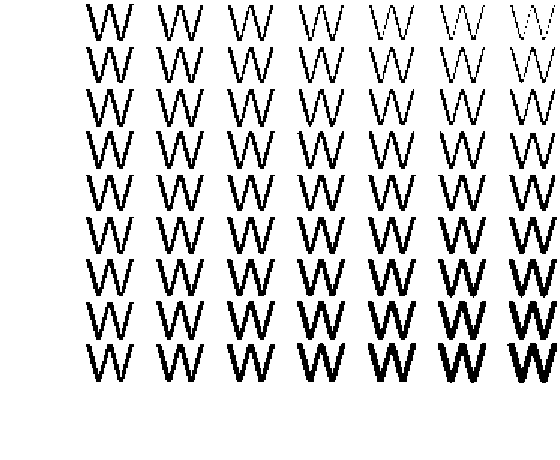
\includegraphics[width=4in,height=\textheight]{figs/figure.pdf}

\subsection{Tables}\label{tables}

Table~\ref{tbl-CSSSM} shows the formatting and labeling for a table. For
complicated formats, you can create a grid table at
https://www.tablesgenerator.com/text\_tables with
\texttt{Use\ reStructuredText\ syntax} selected, or generate an HTML
table (https://quarto.org/docs/authoring/tables.html).

\begin{table}

\caption{\label{tbl-CSSSM}Complexity of Selection and Search in Sorted
Matrices}

\centering{

+:-----------------------------------+:--------------:+:------------------------------------------:+:--------------------:+
\textbar{} \textbar{} Sorted \(X+Y\) \textbar{} Matrix with sorted rows
\textbar{} Matrix with sorted \textbar{}
+-----------------------------------+--------------+---------------------------+--------------+--------------------+
\textbar{} \textbar{} \textbar{} and sorted columns \textbar{} columns
\textbar{}
+-----------------------------------+--------------+---------------------------+--------------+--------------------+
\textbar{} \textbar{} \(|X|=|Y|=n\) \textbar{} \(n \times m\),
\(m \leq n\) \textbar{} \(n \times n\) \textbar{} \(n \times m\)
\textbar{}
+-----------------------------------+--------------+---------------------------+--------------+--------------------+
\textbar{} \(k = \Theta(mn)\) or \(\Theta(n^2)\) \textbar{}
\(\Theta(n)\) \textbar{} \(\Theta(m\log (2n/m))\) \textbar{}
\(\Theta(n)\) \textbar{} \(\Theta(m \log n)\) \textbar{}
+-----------------------------------+--------------+---------------------------+--------------+--------------------+

}

\end{table}%

Here are two more examples of tables:

\section{Conclusions}\label{conclusions}

\subsection{What have we done so far?}\label{what-have-we-done-so-far}

\subsection{Future directions}\label{future-directions}

The coming revolution in Wabi-sabi-lets offers many opportunities for
further research.

\section{References}\label{references}

\phantomsection\label{refs}
\begin{CSLReferences}{1}{0}
\bibitem[\citeproctext]{ref-mepaper1}
Admirer, Wabi-sabi. 1970. {``An Analysis of Wabi-Sabiism.''}
\emph{Journal of the Advanced Computing Wabi-Sabi} 21 (2): 272--87.

\bibitem[\citeproctext]{ref-mepaper2}
Admirer, Wabi-sabi, Jim Smith, and Jane Doe. 1972. {``Everyday
Wabi-Sabiism.''} \emph{Journal of the Advanced Wabi-Sabi Computing} 23
(4): 272--87.

\bibitem[\citeproctext]{ref-guide}
Graduate College. 2021. {``Standards for Preparation of Dissertations,
Theses \& Projects.''}

\bibitem[\citeproctext]{ref-wsbook1}
Great, Wabi-sabi The. 1922. \emph{The World According to Wabi-Sabi}.
Wabi-sabiland: NoWabi-sabi Press.

\bibitem[\citeproctext]{ref-wsbook2}
---------. 1952. \emph{The World Without Wabi-Sabi}. Wabi-sabiland:
NoWabi-sabi Press.

\bibitem[\citeproctext]{ref-mainrepo}
Jain, Amit. 2025. {``Style Files for PhD Dissertation or m.s. Thesis or
Project.''}
\url{https://github.com/BoiseState/thesis-dissertation-template}.

\end{CSLReferences}

\appendix

\section{Timing Measurements}\label{app-Timing}

Here is Appendix A. See Appendix (\textbf{app-Setup?}) for the
experimental setup.

\section{Experimental Setup}\label{app-Setup}

Here is Appendix (\textbf{app-Setup?}).

\finish

% The main text of the work ends here; the remaining text is back matter.
\backmatter

% There are different bibliography styles; 'plain' is used for theses.
\bibliographystyle{plain}


\end{document}
